We identify candidate exoplanet hosts by examining the \textit{Hipparcos}-\textit{Gaia} Catalog of Accelerations presented in \cite{2021ApJS..254...42B} created using the \textit{Gaia} DR3 catalog. We select stars with a $>4\sigma$ proper motion anomaly, combining the significance of the three pairs of proper motions. We exclude known close binaries reported in the Washington Double Star Catalog (WDS) \citep{2001AJ....122.3466M} or the Ninth Catalog of Spectroscopic Binary Orbits (SB9) \citep{2004A&A...424..727P} and stars with obvious companions in archival imaging data. Of the remaining stars, we reject those whose astrometric signal is consistent with a stellar companion between $0.1-1.0''$. We determine the allowed combinations of companion mass and orbital period using the rejection sampling algorithm described in detail in \cite{2023A&A...672A..94D}. We compare simulated astrometric measurements from the simulated photocenter motion caused by an orbiting companion to the observed accelerations. \rev{We use the scan timings and scan angles of the \textit{Hipparcos} and \textit{Gaia} satellites to forward model the position and proper motion of the photocenter measured by the two missions. The photocenter motion is modeled as a combination of the linear motion of the system through space and the orbit of the primary star about the system barycenter.} Figure \ref{dot_ex} shows an example of the allowed mass-period parameter space for a star in our sample (HIP 669) based on the observed astrometric acceleration.

\begin{figure*}[hb!]
\centering
 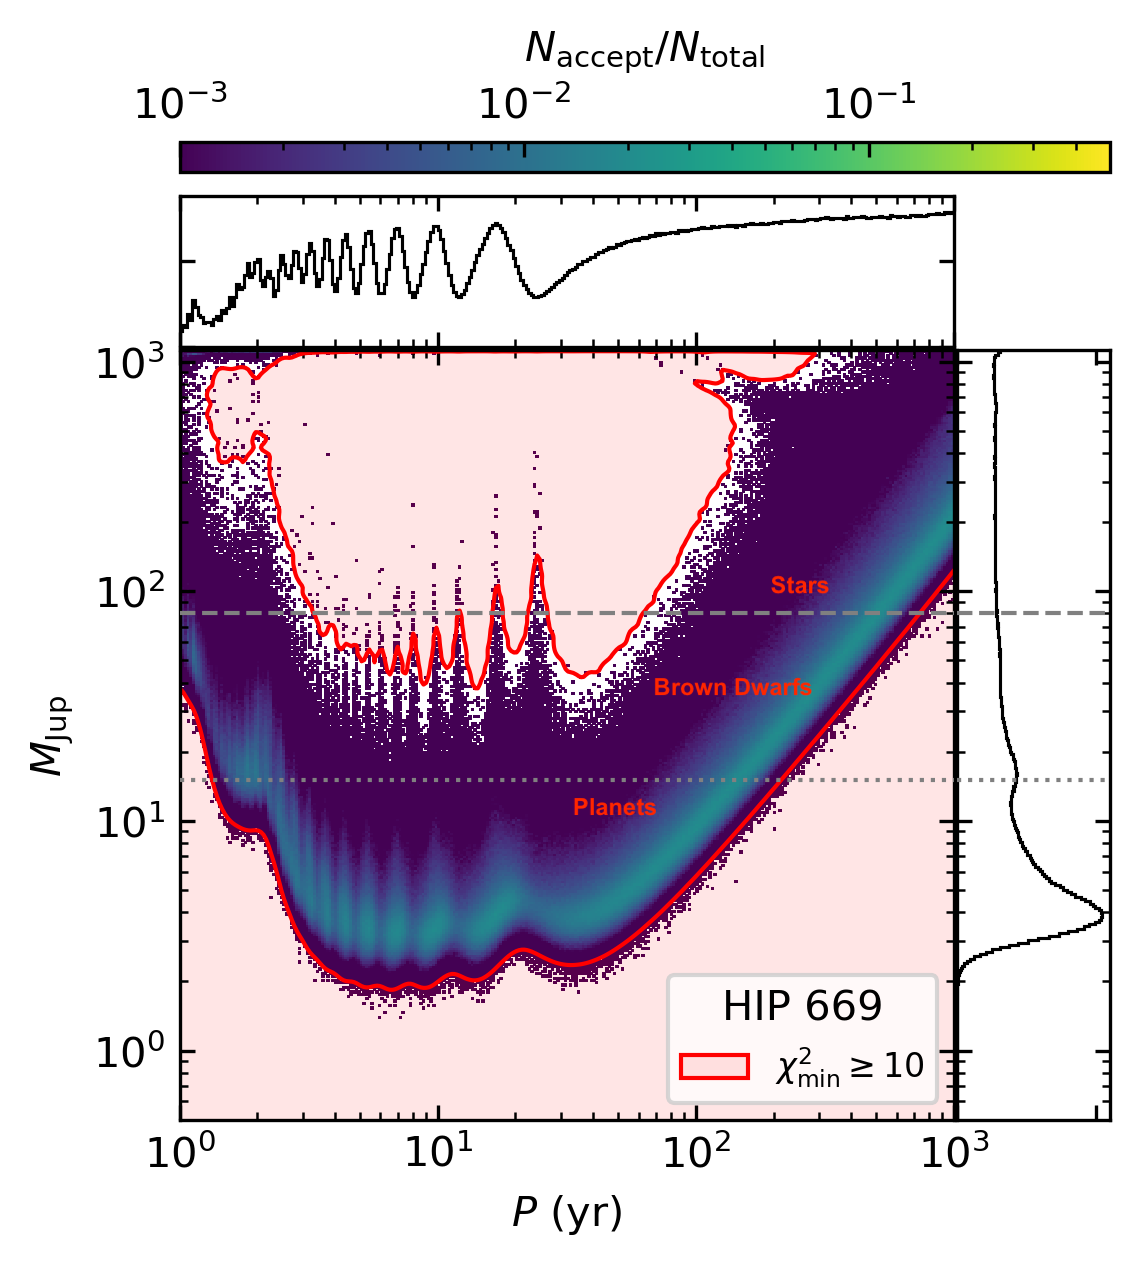
\includegraphics[scale = 0.25]{HIP000669-acceptance.png}
  
 \caption{Results from rejection sampling of combined \textit{Hipparcos} and \textit{Gaia} DR3 astrometry show the possible companion mass-period combinations responsible for the observed acceleration of HIP 669. Candidate companions include stellar binaries, brown dwarfs, and wide-separation giant planets. The near-infrared contrast of these substellar companions depends on the age of the star. }
 % The red dots represent angular separations accessible with current ground-based direct imaging techniques.
 \label{dot_ex}
\end{figure*}
\begin{figure*}[ht!]
\centering
 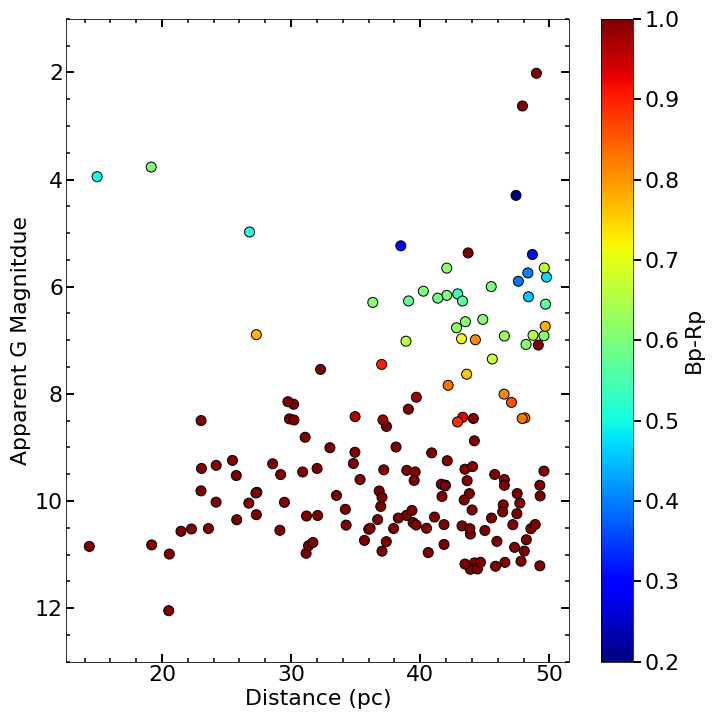
\includegraphics[scale = 0.35]{G_dist_bmr.png}
  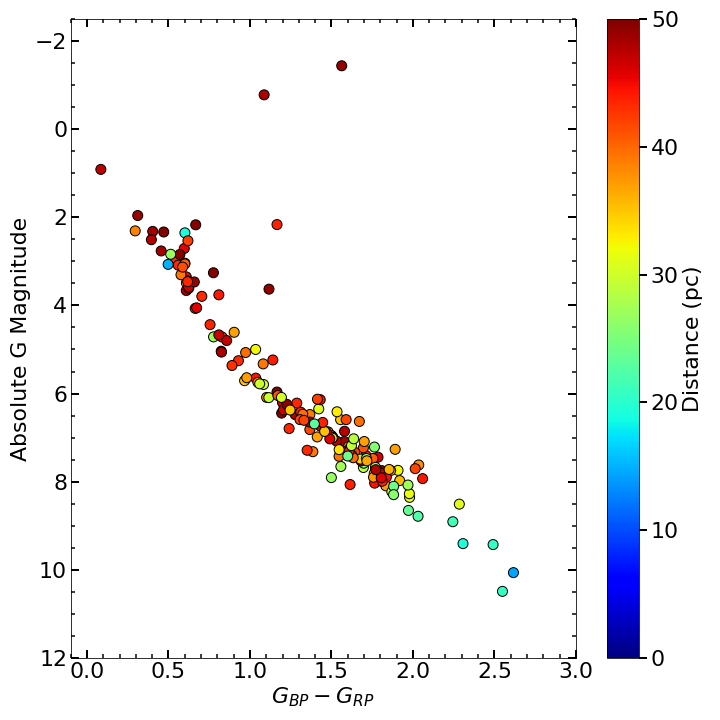
\includegraphics[scale = 0.35]{bmr_G_dist.png}
 \caption{{\bf Left:} Apparent \textit{Gaia} G magnitude of the accelerating stars as a function of distance. {\bf Right:} Color-magnitude diagram of the sample. The median of our sample is $G_{BP}-G_{RP} = 1.4$ ($\sim$K5), 41.5 pc, and $G=9.6$. Our sample covers a wide range of spectral types, so we require a variety of age tracers to derive ages for each star. }
 \label{sample}
\end{figure*}


We limit our sample to stars observable from Apache Point Observatory (APO), i.e. stars with declinations $>-30^{\circ}$. We also limit the sample to stars within 50 pc to maximize the angular separation between the star and the potential companion to maximize the chance of the companion being directly imaged. We do not include stars that have archival radial velocities (e.g. from ESO/HARPS or Keck/HIRES). Figure \ref{sample} shows the distance, color, and magnitudes of our sample. The majority of our sample is between 30-50 pc with apparent G magnitudes between 6 and 11.



 
 Age posteriors for lithium and $R^{'}_{HK}$ from \texttt{BAFFLES} \citep{2020ApJ...898...27S} are calculated as a function of $B-V$. We adopt the $B-V$ values and associated errors that are reported in the \textit{Hipparcos} catalog \citep{1997A&A...323L..61V}. Five stars in our sample (HIP 33368, HIP 46385, HIP 63661, HIP 69860, and HIP 81655) do not have a $B-V$ reported in the \textit{Hipparcos} Catalog. An additional five stars (HIP 9067, HIP 111976, HIP 59953, HIP 1068, and HIP 1771) have very high uncertainties ($\sim$0.5 magnitudes) on their reported B-V colors in the \textit{Hipparcos} catalog. We derive $B-V$ for these targets by fitting a relation to the $B-V$ / $G_{BP}-G_{RP}$ color-color plot (Figure \ref{bmv} in Appendix). We use the $B-V$ values from the \textit{Hipparcos} Catalog \citep{1997A&A...323L..61V} and the $G_{BP}-G_{RP}$ values from \textit{Gaia} DR3 \citep{2023A&A...674A...1G}. We filter the \textit{Gaia} catalog for all stellar entries that were cross-matched to \textit{Hipparcos} by the \textit{Gaia} team, merged the \textit{Hipparcos}/\textit{Tycho} data, we exclude variable stars, and then apply the following filters: $RUWE \leq 1.6$, $Gmag<13$, $Gmag_{err}<0.01$, $Hpmag_{err}<0.1$, $(B-V)_{err}<0.1$, $B-V\neq0.0$, and $B-V<2.0$.

 We find the best-fitting relationship is
 \begin{equation}
 B-V = -0.102(G_{BP}-G_{RP})^{4} + 0.226(G_{BP}-G_{RP})^{3}+0.017(G_{BP}-G_{RP})^{2}+0.688(G_{BP}-G_{RP})+0.002  
\end{equation} Based on the scatter in the relationship, we adopt a 0.1 magnitude uncertainty on the derived $B-V$ colors.
 
 Gyrochronological age posteriors from \texttt{gyro-interp} depend on effective temperature \citep{2023ApJ...947L...3B}. We determine effective temperatures for our sample by interpolating the grid from \cite{2013ApJS..208....9P} to the measured \textit{Gaia} $G_{BP}-G_{RP}$ colors. To estimate the uncertainty on the effective temperature we find the range of effective temperatures corresponding to the range of $G_{BP}-G_{RP}\pm0.1$.


%\subsection{Data Acquisition}

To measure lithium equivalent widths and $R^{'}_{HK}$, we obtain spectra using the Astrophysical Research Consortium Echelle Spectrograph (ARCES) on the APO 3.5 meter telescope. ARCES is a multi-use spectrograph with an average spectral resolution $R = \frac{\Delta\lambda}{\lambda} = 35,000$ covering 3,200 \r{A} to 10,000 \r{A} \citep{2003SPIE.4841.1145W}. We achieve SNRs between $\sim20$ for our faintest targets and $\sim200$ for our brightest stars.
The observing campaign began in October 2020 and is ongoing. We aim to observe each star at least three times over several months to years so that we can vet for binaries, which we will discuss in detail in future work. As of writing, we have observed each star at least once and 98 out of the 166 stars at least three times. We reduce the data using the python package, \texttt{pyvista}\footnote{https://pyvista.readthedocs.io/}. Each spectrum is bias-corrected, extracted, flat-fielded, and continuum-corrected. Wavelength solutions are extracted from the ThAr taken nearest in time to the science frame and are then applied to the science spectrum.  

We measure rotation periods from $TESS$ light curves reduced with the SPOC pipeline  \citep{2016SPIE.9913E..3EJ}. All light curves with cadences between 20-1800s are downloaded from the Mikulski Archive for Space Telescopes (MAST). We found light curves for 129 of our sample stars and identify periodic signals in the light curves of \rev{34} of these 129 stars.